\documentclass{standalone}
\usepackage{tikz}
\usepackage{pgfplots}

\pgfplotsset{
    compat=newest,
}

\begin{document}
    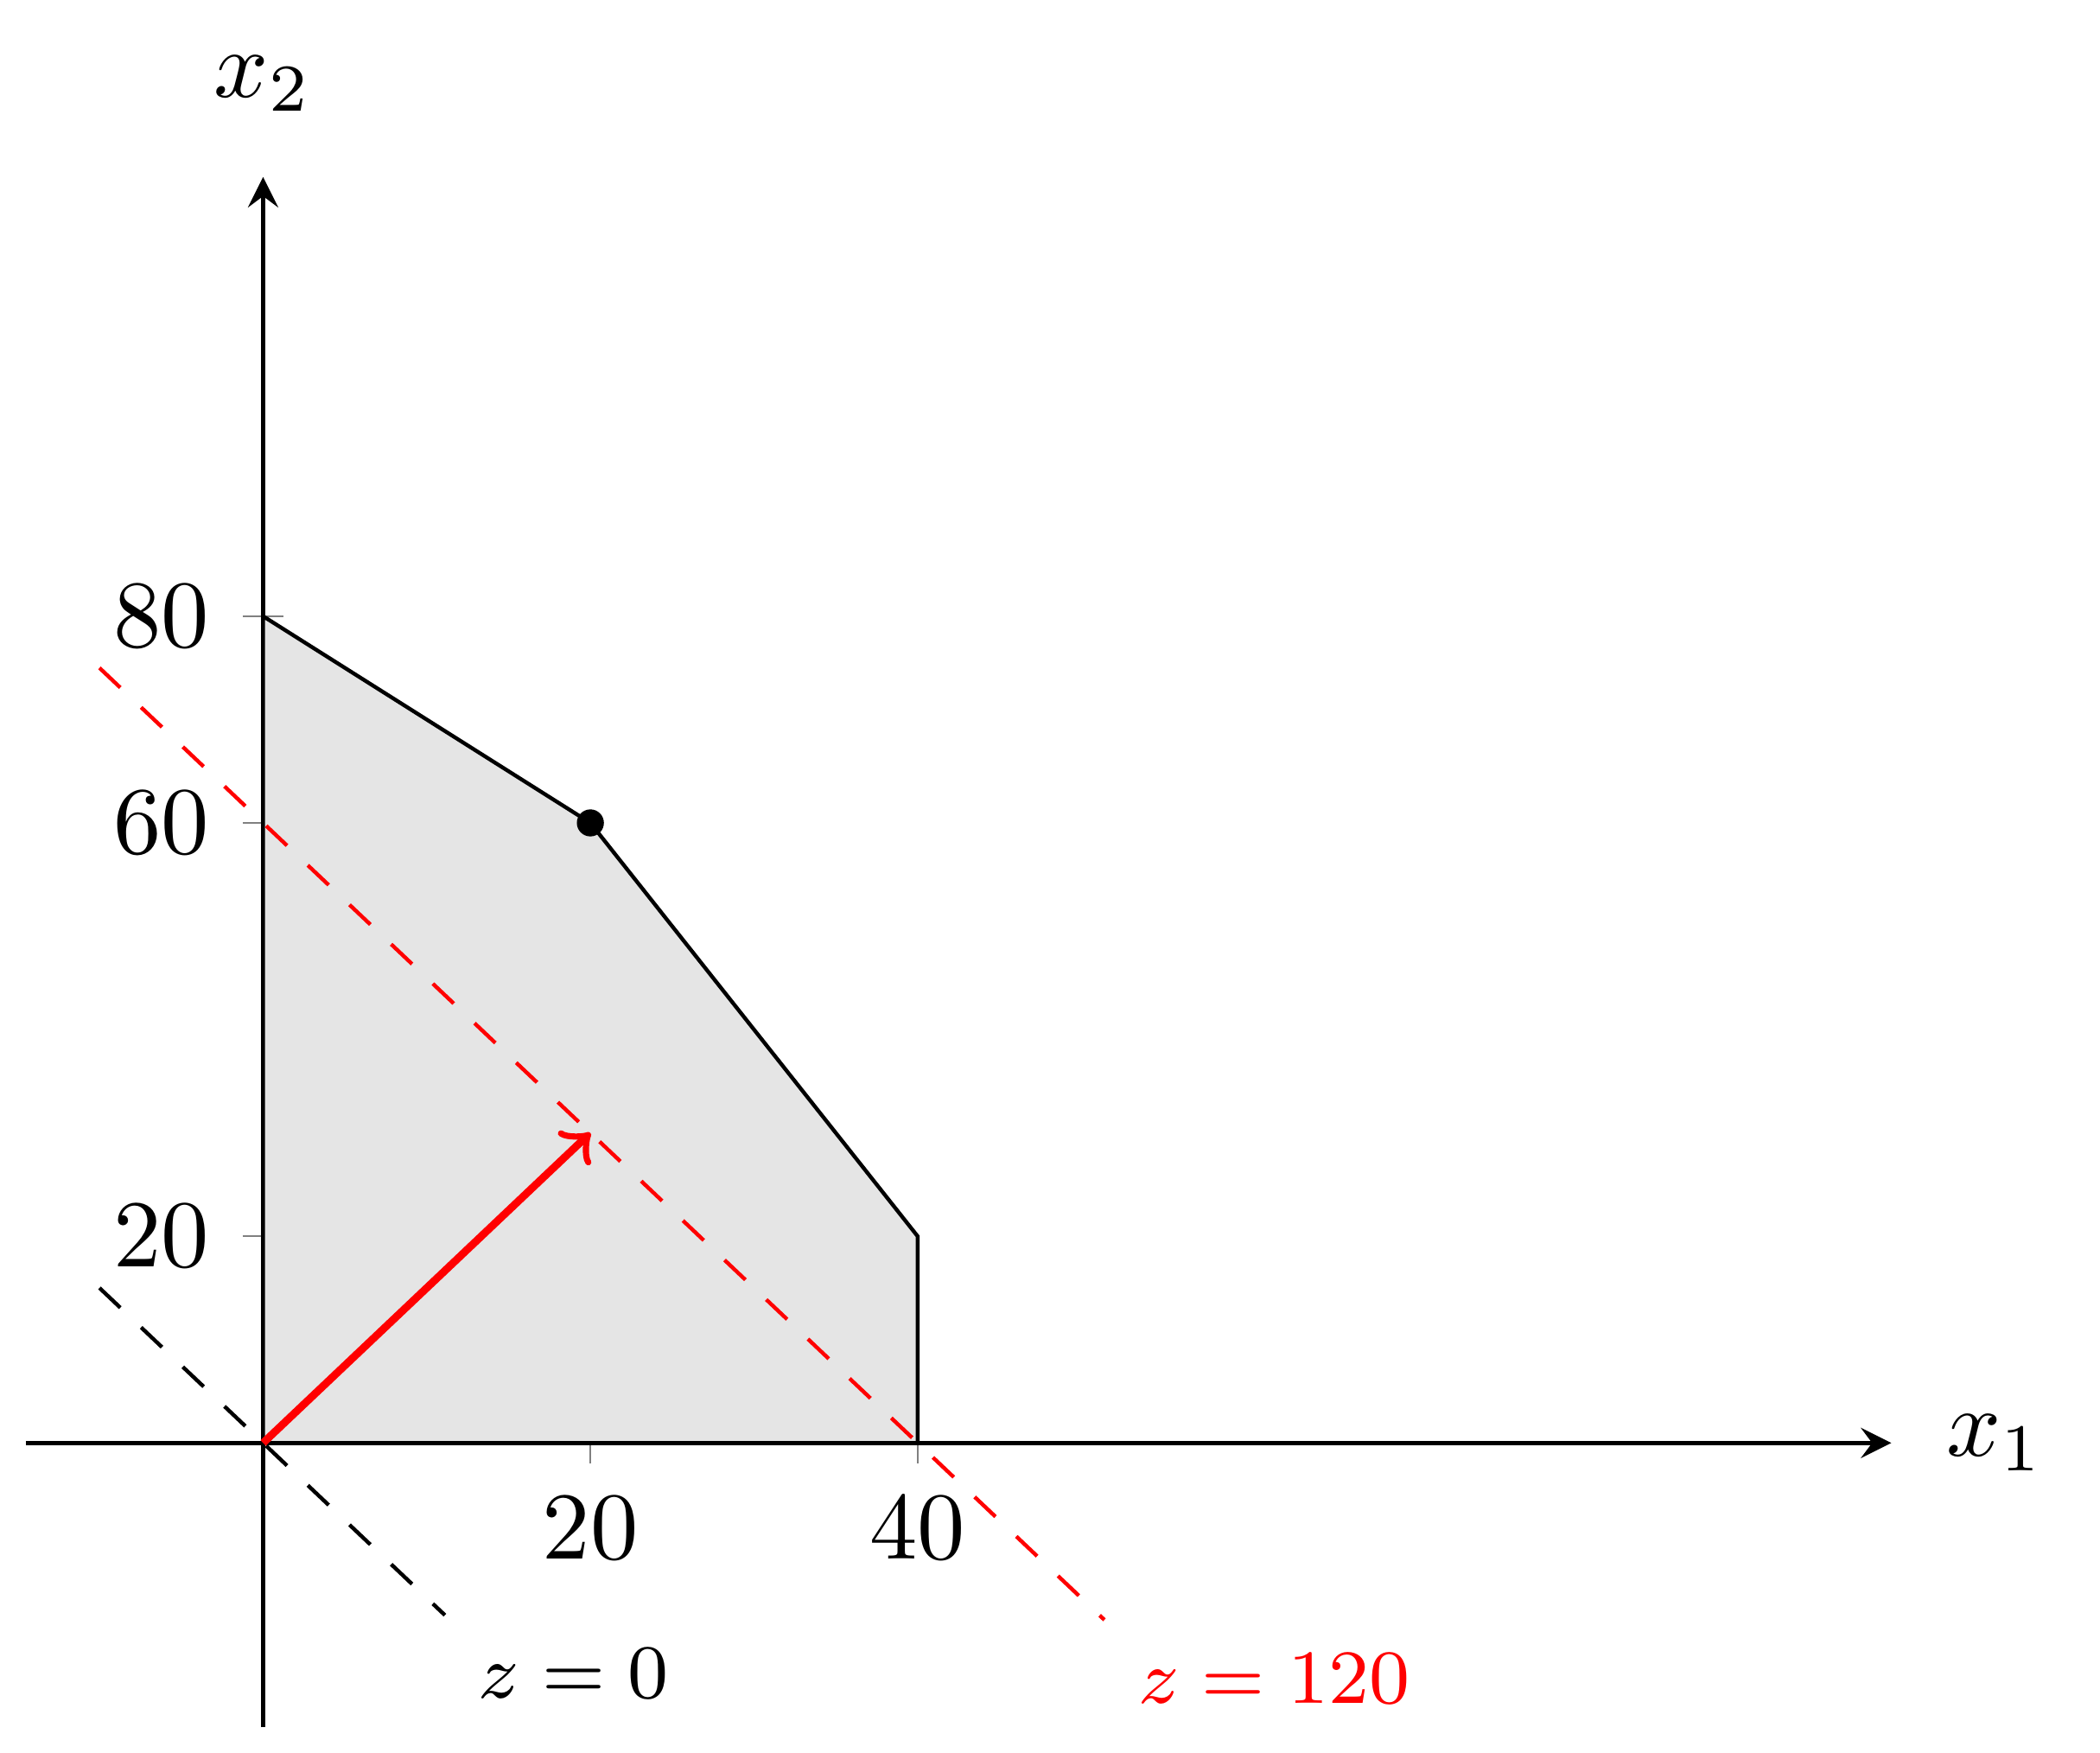
\begin{tikzpicture}[scale=4]
        \begin{axis}[
            axis lines=middle,
            ylabel=$x_2$,
            xlabel=$x_1$,
            every axis x label/.style={
                at={(ticklabel* cs:1.1)},
                anchor=east,
            },
            every axis y label/.style={
                at={(ticklabel* cs:1.1)},
                anchor=north,
            },
            xmin=-5, ymin=-15,
            xmax=90, ymax=110,
            domain=-10:85,
            samples=100,
            xtick={0,20,40},
            ytick={0,20,60,80},
            enlargelimits=true,
        ]
            \coordinate (A) at (0, 0);
            \coordinate (B) at (40, 0);
            \coordinate (C) at (40, 20);
            \coordinate (D) at (20, 60);
            \coordinate (E) at (0, 80);

            \fill[gray!20] (A) -- (B) -- (C) -- (D) -- (E) -- cycle;
            \draw (A) -- (B) -- (C) -- (D) -- (E) -- cycle;
            \draw (D) node[circle, fill, inner sep=1pt]{};

            \addplot[dashed, restrict y to domain=-18:105] {0.5*(0 - 3*x)} node[pos=1, below right]{\footnotesize{$z = 0$}};
            \addplot[red, dashed, restrict y to domain=-18:105] {0.5*(120 - 3*x)} node[pos=1, below right]{\footnotesize{$z = 120$}};
            \draw[->, red, thick] (A) -- (20, 30);
        \end{axis}
    \end{tikzpicture}
\end{document}
